\documentclass{standalone}
\usepackage{xcolor,amsmath,amssymb,amsfonts}
\usepackage{fontspec}
\usepackage[T1]{fontenc}
\usepackage[tt=false, type1=true]{libertine}
\usepackage[libertine]{newtxmath}

\usepackage{tikz}
\usetikzlibrary{arrows.meta}
\definecolor{red}{HTML}{c63a44}
\begin{document}

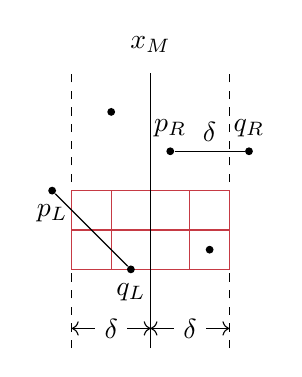
\begin{tikzpicture}[dot/.style={circle,fill,inner sep=1pt}]
\node[dot]at(1,3){};
\node[dot]at(2.25,1.25){};
\node[dot,label=$p_R$]at(1.75,2.5)(pr){};
\node[dot,label=$q_R$]at(2.75,2.5)(qr){};
\node[label=$x_M$]at(1.5,3.5)(x){};
\draw[dashed](0.5,0) -- (0.5,3.5) (2.5,0) -- (2.5,3.5);
\foreach\x in{0.5,1.5}{
    \draw[<->](\x,0.25) -- ++(0.5,0)node[fill=white]{$\delta$} -- ++(0.5,0);
}
\draw[red](0.5,1.5)--(2.5,1.5) (0.5,2)rectangle(2.5,1);
\foreach\x in{1,1.5,2}{
    \draw[red](\x,1)--(\x,2);
}
\node[dot,label=below:$p_L$] at(0.25,2)(pl){};
\node[dot,label=below:$q_L$] at(1.25,1)(ql){};
\draw (pr) edge node[above]{$\delta$} (qr) (ql) edge (pl) (1.5,0) edge (1.5,3.5);
\end{tikzpicture}

\end{document}